\section{La entropía como medida del desorden}
\label{sub:entropiaShannon}

Para ver la cantidad de información que nos aporta cada palabra se hará una introducción a la teoría de la información, específicamente
los conceptos que introdujo Claude Shannon \cite{shannon2001mathematical,abramson1963information}.
Para entender estos conceptos es útil tener una descripción matemática del mecanismo que genera la información. Para eso se define a 
la \textit{fuente} que emite señales de un alfabeto $ S = \{s_1, s_2, \dotsc s_n\}$ de acuerdo a una función de probabilidad fija.
Si la fuente emite señales estadísticamente independientes decimos que es una \textit{fuente de memoria nula} y un símbolo $s$ está completamente determinado por el alfabeto $S$ y las probabilidades $p_1, p_2, \dots , p_n$.


% Se puede calcular la información promedio provista por una fuente de memoria nula de la siguiente manera: si el símbolo $s_i$ ocurre, obtenemos una cantidad de información igual a $I(s_i) = -\log(p_{s_i})$.
% Luego, se define a la entropía como 

% \begin{equation}
%     {\displaystyle \mathrm {H} (S)=\mathbb{E} [\mathrm {I} (S)]=\mathbb{E} [-\log(\mathrm {P} (S))]} = -\sum\limits_{i=1}^{n} p_{s_i} \log(p_{s_i})
% \end{equation}



% Los símbolos con menor probabilidad son los que aportan más información. Esto va de la mano con nuestra intuición ya que si entendemos a los símbolos como palabras de un texto, las palabras más utilizadas como \textit{de} o \textit{que} aportan menos información que la palabra \textit{celular}. 


Luego, sea $\mathbf{p}=(p_1,\ldots, p_n)$ un vector de probabilidad puntual. Es decir, $p_i\geq 0$ y $\sum_{i=1}^np_i=1$. 
Definimos la entropía de $\mathbf{p}$ siendo
\begin{equation}
H(\mathbf{p})=-\sum_{i=1}^n \log(p_i)p_i.
\end{equation}

De esta forma, la funci\'on  $H$ satisface las siguientes propiedades: 

\begin{itemize}
\item[(i)] $H(\mathbf{p})=0$ si y solo si $\mathbf{p}$ esta concentrada en un unico punto: existe $i$ tal que $p_i=1$ y $p_j=0$, para todo $j\not=i$. 

\item[(ii)] La funci\'on $H$ se maximiza tomando $\mathbf{p}$ equiprobable: 
$p_i=1/n$, para todo $i$. 

\end{itemize}

% Dado que la entropía es máxima cuando los eventos de $X$ son equiprobables, se suele decir que es una medida del desorden.

Tenemos entonces que la m\'axima entrop\'ia se realiza cuando todos los elementos tienen igual probabilidad de ocurrir. Ninguno de ellos es m\'as probable que otro. No hay como predecir un valor en particular. En tal caso, decimos que el desorden es m\'aximo. Por el contrario, cuando la probabilidad se concentra en un \'unico punto, estamos en un sistema destermin\'istico: orden total. En este sentido es que $H$ es una medida de \textit{orden} del sistema. Mayor entrop\'ia dice de m\'as desorden; entendiendo desorden como \textit{aleatoriedad completamente impredescible - distribuci\'on  uniforme}.  


\section{Tablas y Gráficos}
\label{sub:tablas}


\begin{table}[ht]
\centering

\begin{tabular}{ c c }
\toprule
Palabra & Cantidad de Ocurrencias \\ 
\midrule
que     & 7509160                 \\
de      & 6527014                 \\
a       & 4962492                 \\
la      & 4913854                 \\
no      & 4177810                 \\
me      & 4101998                 \\
y       & 3838370                 \\
el      & 3773455                 \\
en      & 2969783                 \\
te      & 2060662                 \\
se      & 1976027                 \\
un      & 1863075                 \\
es      & 1825892                 \\
con     & 1799979                 \\
lo      & 1712189                 \\
mi      & 1643777                 \\
por     & 1553382                 \\
los     & 1498941                 \\
para    & 1398757                 \\
las     & 1212452                 \\
\bottomrule
\end{tabular}
\caption{Cantidad de apariciones de las 20 palabras más frecuentes.}
\label{tab:palabrasMasOcurrentes}
\end{table}


\begin{table}
\centering
{%
\begin{tabular}{|c|c|c|c|}
\hline
\multicolumn{4}{|c|}{Conjunto de Provincias} \\ \hline
\hline
Salta-Jujuy & Mendoza-San Juan & Chubut-Santa Cruz-T. Del Fuego & Chaco-Corrientes-Formosa   \\ \hline
tribuno     & mza              & austral                        & anga                       \\
salteño     & zonda            & chilote                        & teresss                    \\
orán        & secamente        & calafa                         & músicas                    \\
tartagal    & sanjuaninos      & chilota                        & argela                     \\
salteña     & sanjuanino       & palmaso                        & angaaa                     \\
martearena  & asar             & vueltines                      & olo                        \\
oran        & tomba            & riviera                        & cuchale                    \\
yuto        & queras           &                                & corrientesss               \\
purmamarca  & traica           &                                & angá                       \\
yutos       & sopaipillas      &                                & cts                        \\
gorriti     & ardente          &                                & correntinas                \\
quijano     & secamentes       &                                & iburrr                     \\
tabacal     & jáchal           &                                & cheraa                     \\
desentierro & virreina         &                                & cheraá                     \\
huaico      & tombaaa          &                                & bofill                     \\
pichanal    & mansooo          &                                & receppp                    \\
diableros   & tombino          &                                &                            \\
bandy       & parisi           &                                &                            \\
aramayo     & asadaaa          &                                &                            \\
ñaño        &                  &                                &                            \\
colque      &                  &                                &                            \\
urkupiña    &                  &                                &                            \\
juy         &                  &                                &                            \\
guachipas   &                  &                                &                            \\ \hline
\end{tabular}%
}
\caption{Palabras cubiertas sobre el 80\% de las ocurrencias totales por el conjunto de provincias a partir de las 5000 palabras más contrastivas (de acuerdo al valor de la información).}
\label{tab:palabrasRegiones}
\end{table}

\begin{figure}[ht]
\centering
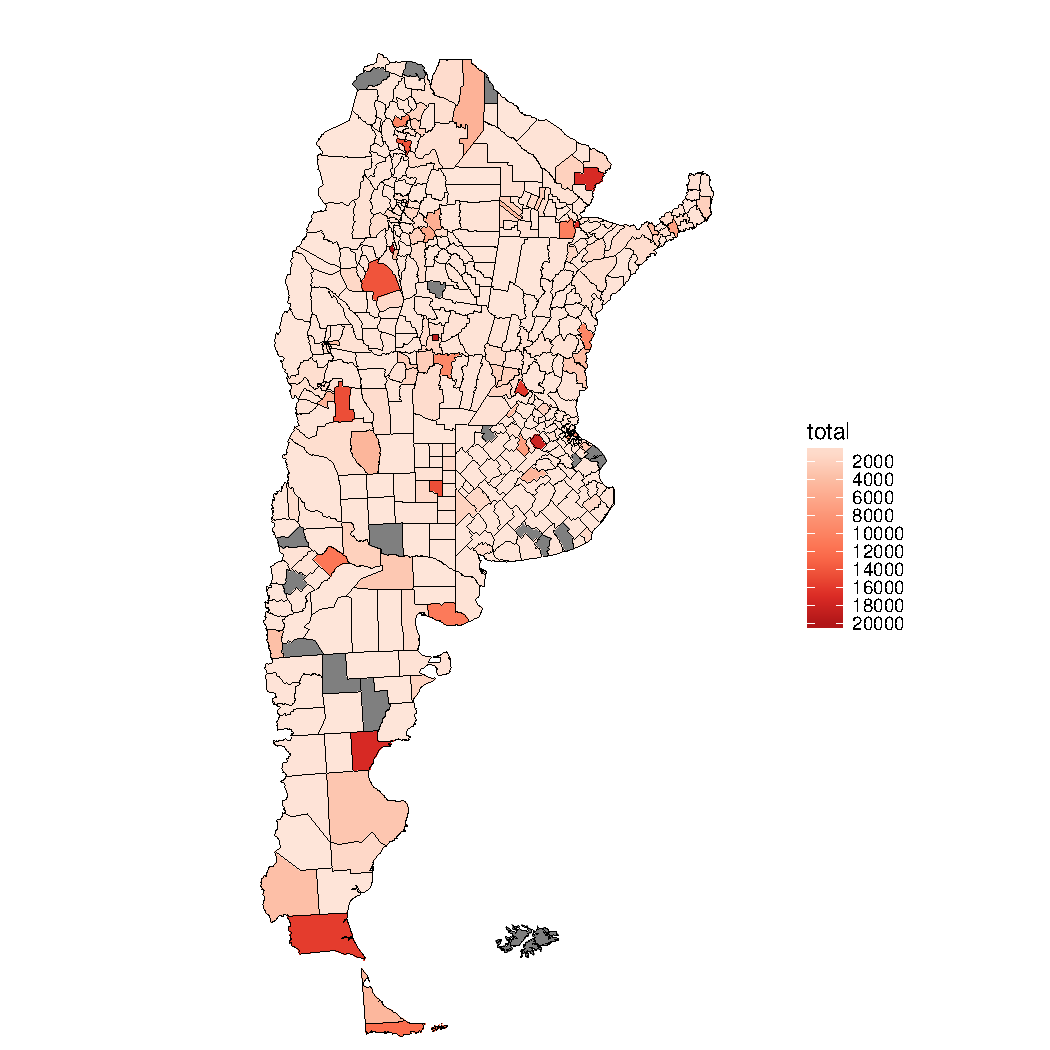
\includegraphics[width=1.0\textwidth]{./images/mapaGPS.pdf}
\caption{Mapa con la distribución de los tuits que incluyeron sus coordenadas geográficas. } 
\label{fig:mapaGPS} 
\end{figure}